\documentclass[../main.tex]{subfiles}
\graphicspath{{\subfix{../images/}}}
\begin{document}


Vlastnost aproximace $z_h$:
\begin{equation}
    z_h(x_J) = \sum_{j=1}^D \alpha_j \phi_j (x_j)= \sum_{j=1}^D \alpha_j \delta_{jJ} = \alpha_J
\end{equation}

\begin{remark}[Zpracování zaoblených částí $\partial\Omega$]
    \begin{figure}
        \centering
        \begin{subfigure}[bt]{0.5\textwidth}
            \centering
            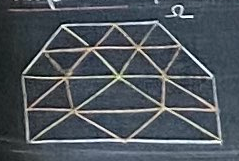
\includegraphics[width=1\textwidth]{images/diskretizace.png}
            \caption{Diskretizace $\Omega$ \hfill\break Bíla je původní oblast,\hfill\break žlutě základní rozdělení,\hfill\break červeně zjemnění \hfill}
        \end{subfigure}
        \hfill
        \begin{subfigure}[t]{0.5\textwidth}
            \centering
            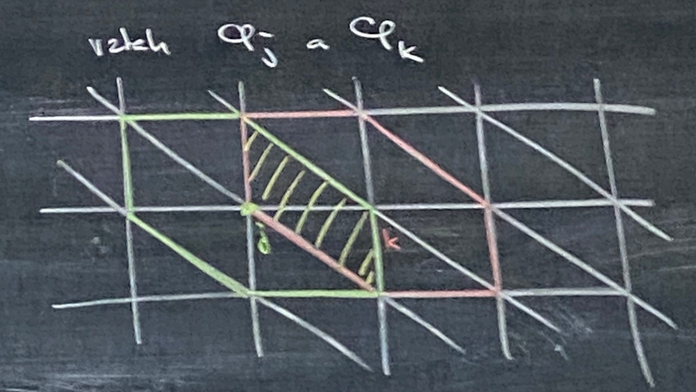
\includegraphics[width=1\textwidth]{images/vztahphi.png}
            \caption{Vztah $\phi_j$ a $\phi_k$}
        \end{subfigure}
    \end{figure}

Buď se modré částí z \ref{obrazek} se převedou pomocí konformních zobrazení na $\triangle$ nebo tvar $\Omega$ aproximujeme polygonem, viz \ref{dalsi obrazek}
\end{remark}

\begin{example}[MKP v 1D]
    Okrajová úloha (tj. \refI)
    \begin{equation}
        -(p(x)u')' + q(x) u = f(x), \text{na} (a,b)
    \end{equation}
    \begin{equation}
        u(a) = 0, u'(b) = 0
    \end{equation}

    Variační formulace (tj. \refII):
    \begin{equation}\label{variacniformulace1d}
        a(u,v) = \int_a^b p(x)u'v' + q(x)uv \ dx, F(v)=\int_a^b f(x)v \ dx \implies V = \{v\in\mathbb{W}_2^{(1)}(a,b)| v|_{x=a} = 0  \}, a(u,v) = F(v) \forall v\in V
    \end{equation}

    MKP pro \ref{variacniformulace1d}: (a,b) dělíme stejnoměrně (viz obrázek \ref{jestejednenobrazek}) kde $h=\frac{b-a}{D}$

    Dostáváme funkce $\phi_k$ jako v obrázku \ref{jesetedalsiobrazek}

    Z toho vidíme že platí:
    \begin{equation}
        a(\phi_j, \phi_k)=
        \begin{cases}
          0 & \text{pro}\ l\neq j-1, j, j+1 \\
          \int_{x_{j-1}}^{x_{j+1}} \\
          \int_{x_{j-1}}^{x_{j}} & \text{pro} l=j-1\\
          \int_{x_{j}}^{x_{j+1}} & \text{pro} l=j+1
        \end{cases}
      \end{equation}
    
    Tvar bazické funkce: 
    \begin{equation}
        \phi_j(x) = 
        \begin{cases}
            \frac{x-x_{j-1}}{x_j - x_{j-1}} & \text{na} <x_{j-1}, x_j> \\
            \frac{x_{j+1}-x}{x_{j+1} - x_{j}} & \text{na} <x_{j}, x_{j+1}> \\
            0 & \text{jinak}
        \end{cases}
    \end{equation}


Pak:
\begin{equation}
    a(\phi_j, \phi_j) = \int_{x_{j-1}}^{x_j} p(x) \left( \frac{1}{x_j - x_{j-1}} \right)^2 + q(x) \left( \frac{x-x_{j-1}}{x_j-x_{j-1}} \right)^2 \ dx + \int_{x_j}^{x_{j+1}} p(x) \left( \frac{-1}{x_{j+1} - x_j} \right)^2 + q(x) \left(\frac{x_{j+1}-x}{x_{j+1} - x_j}\right)^2 \ dx 
\end{equation}

\begin{equation}
    a(\phi_j, \phi_{j-1}) = \int_{x_{j-1}}^{x_j}  p(x) \left( \frac{1}{x_j - x_{j-1}} \right)  \left( \frac{-1}{x_{j} - x_{j-1}} \right) + q(x) \left( \frac{x-x_{j-1}}{x_j-x_{j-1}} \right) \left( \frac{x_j -x}{x_{j} - x_{j-1}} \right) \ dx
\end{equation}

\begin{equation}
    a(\phi_j, \phi_{j+1}) = \int_{x_{j}}^{x_{j+1}}  p(x) \left( \frac{-1}{x_{j+1} - x_{j}} \right)  \left( \frac{1}{x_{j+1} - x_{j}} \right) + q(x) \left( \frac{x_{j+1}-x}{x_{j+1}-x_{j}} \right) \left( \frac{x - x_j}{x_{j+1} - x_{j}} \right) \ dx
\end{equation}

Použijeme substituci: 

\begin{equation}
    y = \frac{x - x_{j-1}}{x_j - x_{j-1}} \text{na} <x_{j-1}, x_j> \mapsto <0,1>
\end{equation}
\begin{equation}
    y = \frac{x_{j+1} - x}{x_{j+1} - x_{j}} \text{na} <x_{j}, x_{j+1}> \mapsto <0,1>
\end{equation}

Pak: 
\begin{equation}
    a(\phi_j, \phi_j) = \int_0^1 p((x_j - x_{j-1})y + x_{j-1}) \frac{dy}{x_j - x_{j-1}} + \int_0^1 q((x_j - x_{j-1})y + x_{j-1}) y^2 (x_j - x_j-1) \ dy - \int_0^1 p(-(x_{j+1} - x_j)y + x_{j+1}) \frac{dy}{ x_{j+1 - x_j}} - \int_0^1 q(-(x_{j+1} - x_j)y + x_j+1) y^2 (x_{j+1 - x_j}) \ dy
\end{equation}

\begin{equation}
    a(\phi_j, \phi_{j-1}) = - \int_0^1 p((x_j - x_{j-1})y + x_{j-1}) \frac{dy}{x_j - x_{j-1}} - \int_0^1 q((x_j - x_{j-1})y + x_{j-1}) y(1-y) (x_j - x_j-1) \ dy
\end{equation}

\begin{equation}
    a(\phi_j, \phi_{j+1}) = \int_0^1 p(-(x_{j+1} - x_j)y + x_{j+1}) \frac{dy}{ x_{j+1 - x_j}} - \int_0^1 q(-(x_{j+1} - x_j)y + x_j+1) y(1-y) (x_{j+1 - x_j}) \ dy
\end{equation}

Z toho je poznat že matice $a(\phi_j, \phi_l)$ je symetrická
\end{example}

\section{Základní aspekty MKP (Ciarlet str. 38)}
\begin{theorem}[MKP1]
    Množina $\bar{\Omega}$ (z \refI) je rozdělena triangulací $\mathcal{T}_h$ na konečný počet podmmnožin K (oblastí konečných prvků) tak, že 
    \begin{enumerate}
        \item $\bar{\Omega} = \bigcup_{K\in\mathcal{T}_h} \bar{K}$
        \item $(\forall K  \in \mathcal{T}_h)(K\neq\emptyset \text{ a K je oblast})$
        \item $(\forall K_1, K_2 \in \mathcal{T}_h)(K_1 \neq K_2 \implies K_1 \cap K_2 = \emptyset)$
        \item $(\forall K \in \mathcal{T}_h) (\partial K \text{ je Lipschitzovská} )$
    \end{enumerate}
\end{theorem}

\begin{theorem}[MKP2]
    Na každé množině $K\in\mathcal{T}_h$ definujeme vhodné funkce sloužící k aproximaci řešení variační úlohy \refII . Tyto funkce jsou polynomy, nebo "blízké" polynomům
\end{theorem}


\begin{theorem}[MKP3]
    Aproximaci řešení variační úlohy \refII hledáme pomocí bazických funkcí, jejichž nosič je co nejmenší při zachování shodného popisu tvaru těchto funckí. 
\end{theorem}


\begin{definition}[Konečný prvek]
    Nechť \begin{enumerate}
        \item $K \subset \mathbb{R}^n$ je omezená oblast s po částech hladkou hranicí
        \item $\mathcal{P}$ je konečně rozměrný prostor funckí na $\bar{K}$
        \item $\mathcal{N} = \{N_1, ..., N_2\}$ je báze $\mathcal{P}^{\#}$
    \end{enumerate}
    Pak $(K, \mathcal{P}, \mathcal{N})$ se nazývá konečný prvek, $K$ je oblast prvku, $\mathcal{P}$ jsou tvarové funkce a $\mathcal{N}$ uzlové proměnné.

    Báze v $\mathcal{P}$ duální k $\mathcal{N}$ se nazývá nulová báze.
\end{definition}

\end{document}